
\chapter{Grundlegende Komponenten und deren Funktionsweise}

Folgende Funktionalitäten müssen von der Architektur zwingend erfüllt werden, damit Norbert korrekt funktionieren kann:
\begin{enumerate}
	\item Der Newsfeed muss auf dem Client angezeigt werden können.
	\item Norbert muss die gesamten Daten (Einträge, Vorschläge, Emails. etc.) zentral speichern.
	\item Die für den Newsfeeds relevanten Daten müssen von Norbert an die Clients geliefert werden können.
	\item Der Client muss Einträge anlegen/bearbeiten können und auf Vorschläge reagieren können, bzw. seine Aktionen Norbert mitteilen können.
	\item Norbert muss Vorschläge liefern können.
\end{enumerate}
 


\section{Grundlegender Aufbau aus Funktionssicht}


  Die in Grafik \ref{fig: Overview_HLVL} gezeigte Architektur würde die oben genannten Kriterien erfüllen.
  \begin{enumerate}
  	\item Über einen Webbrowser kann der Newsfeed auf den Clients angezeigt werden.
  	\item Norbert hat die gesamten Daten in getrennten Dateien/Ordnern zur Verfügung.
  	\item Über die Kommunikationsschnittstelle kann Norbert die relevanten Daten an den Client liefern.
  	\item Über die Kommunikationsschnittstelle können die Aktionen der Clients Norbert mitgeteilt werden.
  	\item Die Vorschlagslogik berechnet anhand der vorhandenen Daten Vorschläge, welche über die Kommunikationsschnittstelle an den Client geliefert werden.
  	\end{enumerate}

  	
\begin{figure}[H]
\centering
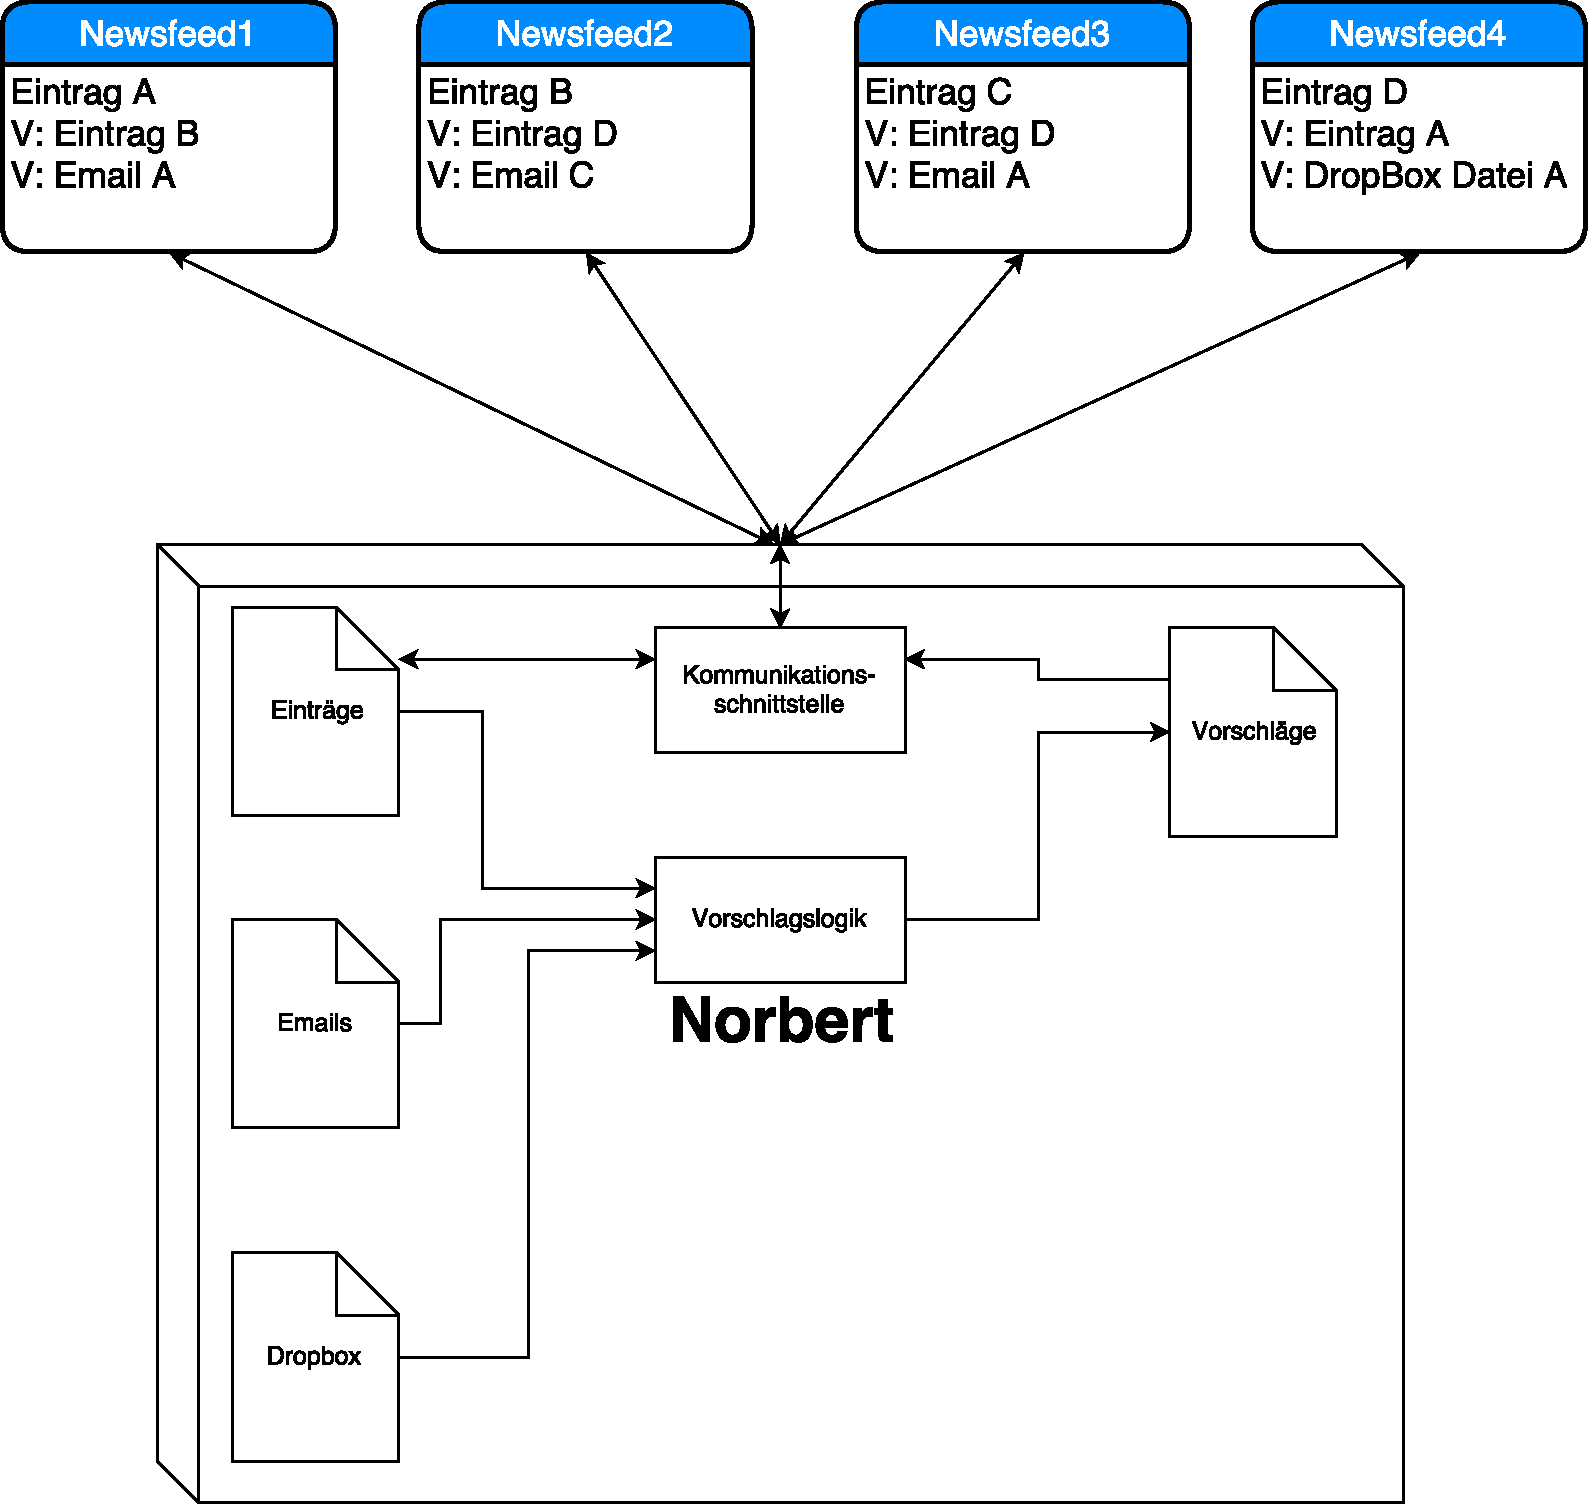
\includegraphics[scale=0.6]{uml-diagramms/overview_hlvl.pdf}
\caption{Grundlegende Funktionalität}
\label{fig: Overview_HLVL}
\end{figure}

Mit dieser Architektur treten aber mehrere Probleme auf:
  	\begin{enumerate}
  	\item Das manuelle Verwalten von Daten in separaten Dateien ist sehr aufwendig und extremst fehleranfällig.
  	\item Der Ablauf interner Prozesse ist nicht definiert und es ist unklar, wie dieser gesteuert wird
  	\end{enumerate}

\section{Datenhaltung}

Das erste Problem kann durch die Verwendung eines Datenbanksystems gelöst werden. Durch eine Datenbank können die Daten zentral verfügbar gemacht werden. Außerdem ist der Zugriff über ein Datenbanksystem weniger fehleranfällig und in der Regel auch effizienter, da die meisten Datenbanksysteme bereits von Haus aus Performanceoptimierungen wie Puffer etc. mitbringen. 
\begin{figure}[H]
\centering
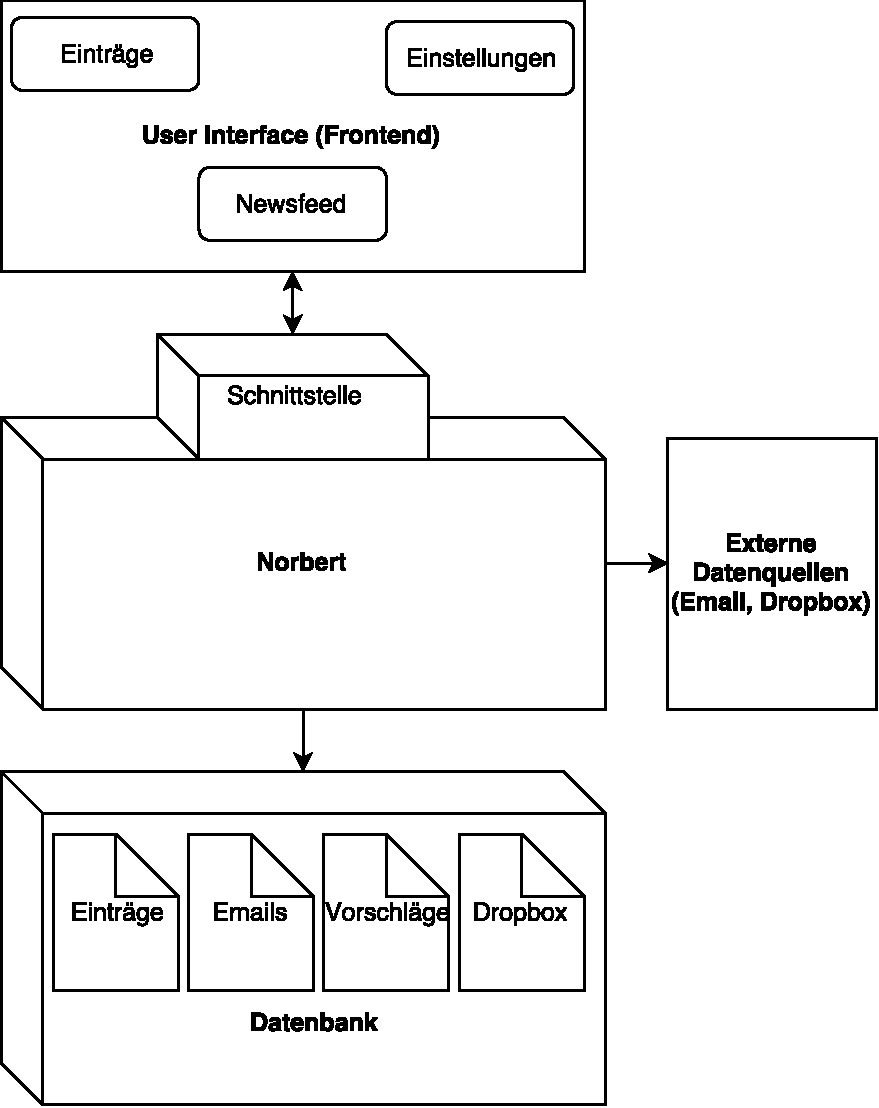
\includegraphics[scale=0.75]{uml-diagramms/daten_hlvl.pdf}
\caption{Kapselung der Daten in einer Datenbank}
\label{fig: DB_HLVL}
\end{figure}

\section{Interne Prozesse}

Das zweite Problem kann durch eine Komponente zur Aufgabenverwaltung gelöst werden. Anstatt Aufgaben wahllos in Echtzeit zu bearbeiten, werden diese zunächst durch die Aufgabenverwaltung in eine Warteschlange eingereiht. Diese Liste an Aufgaben wird dann in regelmäßigen Abständen durch den Core, also die zentrale Logik- und Rechenkomponente, abgearbeitet. Ausnahme hierbei ist das Liefern von Daten an den Client, da dies möglichst schnell erfolgen sollte. Durch das Sammeln von Aufgaben und zyklisches Verarbeiten kann unter anderem die Anzahl seperater Schreibzugriffe auf die Datenbank reduziert werden, wodurch weniger Ressourcen verbraucht werden. Die in Abbildung \ref{fig: Overview_Detail} gezeigte Architektur erfüllt die genannten Anforderungen und löst die in Abbildung \ref{fig: Overview_HLVL} auftretenden Probleme. Die genauere Funktionsweise einzelner Komponenten wird in den folgenden Kapiteln beschrieben.

\begin{figure}[H]
\centering
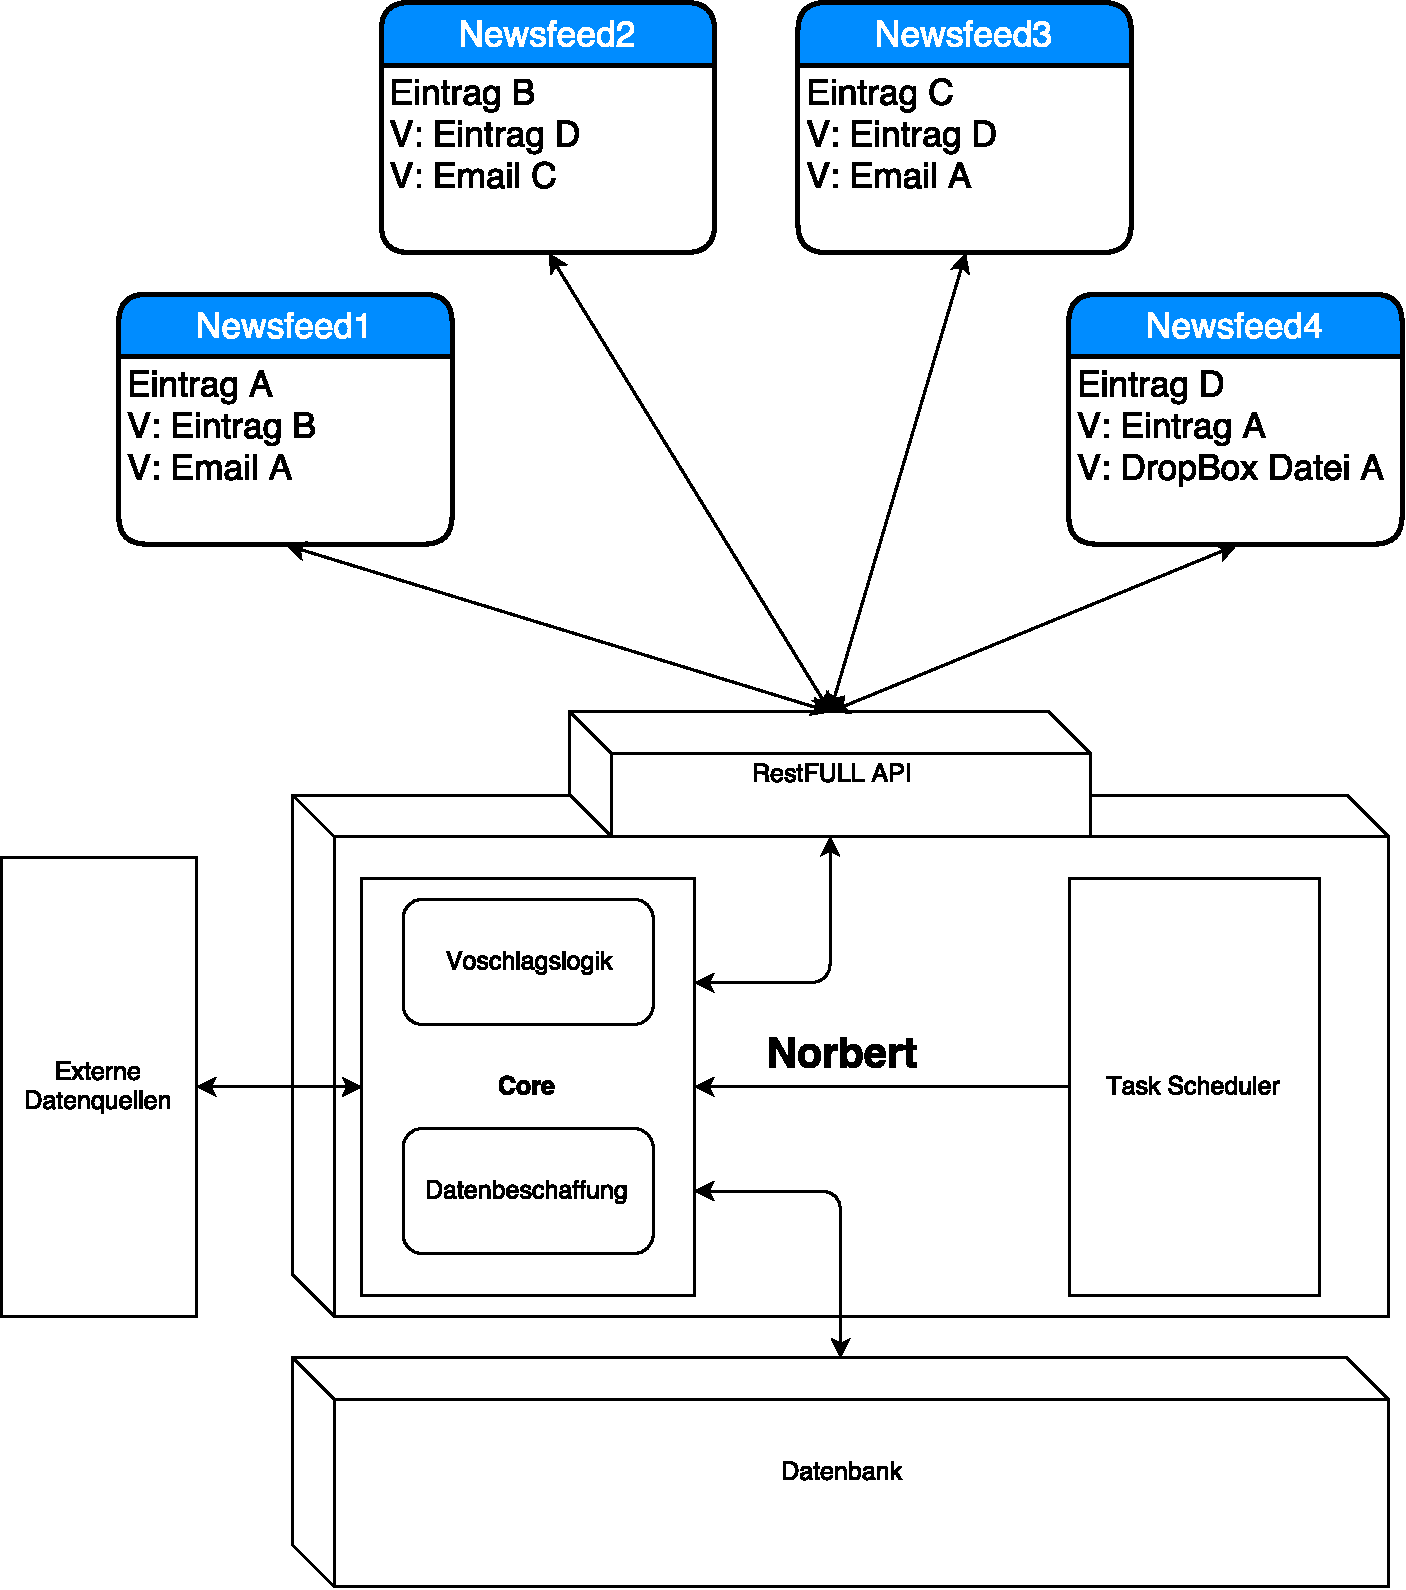
\includegraphics[scale=0.6]{uml-diagramms/overview_detail.pdf}
\caption{Kapselung der internen Prozesse}
\label{fig: Overview_Detail}
\end{figure}




        